% \documentclass[12pt,letterpaper,oneside]{IEEEtran}
\documentclass[12pt,letterpaper,twocolumn]{article}
\usepackage{tikz}
\usepackage{amsmath}
\usepackage{amsfonts}
\usepackage{amssymb}
\usepackage{graphicx}
%\usepackage[left=1in,right=1in,top=1in,bottom=1in]{geometry}

\author{Luis David Licea Torres}
\title{Deriving Circle Formulas from Square Formulas: Relating Spheres, Cubes, and their Cross-sections }
\date{April 11, 2018}

\begin{document}
\maketitle

Let us assume that we do not know anything about circles besides the following equation:
	\begin{equation}\label{eq:formula}
		S = C \cdot\dfrac{\pi}{2D} \mid  s=2r
	\end{equation}
Where \textit{S} stands for the formula of a sphere or circle, \textit{C} stands for the formula of a cube or square, \textit{D} stands for the number of dimensions in the geometric shape, \textit{s} stands for the side length of the square, and \textit{r} stands for the radius of the circle or sphere. If the circle is inscribed in the square, then the length of the square's side will be $s = 2r$ as shown in Figure \ref{fig: side relation}.

\begin{figure}[htbp]
    \centerline
    {
        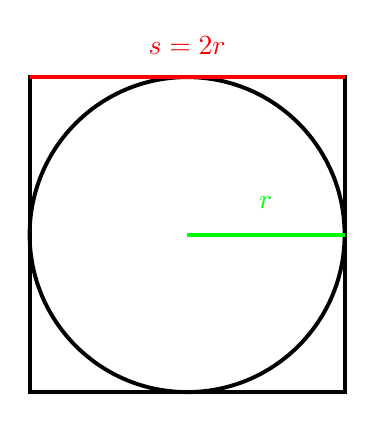
\begin{tikzpicture}
            %\draw (2,2) -- (4,2) node[anchor=west] {r};
            \draw[line width = 0.5mm] (0,0) rectangle (4,4);
            \draw[line width = 0.5mm] (2,2) circle (2);
            \draw[line width = 0.5mm, red] (0,4) -- (4,4) node [label={[xshift=-2cm, yshift=0cm]$s = 2r$}] {};
            \draw[line width = 0.5mm, green] (2,2) -- (4,2) node [label={[xshift=-1cm, yshift=0.05cm]$r$}] {};
        \end{tikzpicture}
    }
    \caption{Illustration of a circle inscribed in a square.}
    \label{fig: side relation}
\end{figure}

The logic for designing formula (\ref{eq:formula}) is simple: as long as the dimensions of a square or a cube are given, the dimensions of its incribed circle or sphere can be calculated. Analyzing 2-dimensionally, squares have a larger area than their inscribed circles because circles are missing four corners; however, the missing area of those four corners is accounted for in equation (\ref{eq:formula}). 

\section*{Applying the Formula}
Equation (\ref{eq:formula}) can be used to find the volume, surface area, area, perimeter (circumference), and lenght (arc length) of spheres and circles. 

\subsection*{Volume}
To see how the equation works, consider the formula for the volume of a cube and the number of dimensions a cube has:
	\begin{align}
		C_{volume} = s^{3} && D =  3
	\end{align}
In order to find the corresponding volume of a sphere inscribed in such cube, we must plug $D$, the number of dimensions, into equation (\ref{eq:formula}), as shown below:
	\begin{align*}
		S_{volume} &= C_{volume} \cdot\dfrac{\pi}{2D} \mid  s=2r \\
		&= s^{3} \cdot\dfrac{\pi}{2\cdot 3} \mid s=2r\\
		&= (2r)^{3} \cdot\dfrac{\pi}{6} \\
		&= \dfrac{8\pi r^{3}}{6} \\
		&= \dfrac{4\pi r^{3}}{3} \\
	\end{align*}

\subsection*{Surface Area}
Consider the formula for the surface area of a cube and the number of dimensions a cube has:
	\begin{align}
		C_{surfaceArea} = 6s^{2} && D =  3
	\end{align}	
Then the corresponding surface area of a sphere inscribed in such cube can be found using equation (\ref{eq:formula}), as shown below:
	\begin{align*}
		S_{surfaceArea} &= C_{surfaceArea} \cdot\dfrac{\pi}{2D} \mid  s=2r \\
		&= 6s^{2} \cdot\dfrac{\pi}{2\cdot 3} \mid s=2r\\
		&= 6(2r)^{2} \cdot\dfrac{\pi}{6} \\
		&= 4\pi r^{2}
	\end{align*}

\subsection*{Area}
Consider the formula for the area of a square (the cross-section of a cube) and the number of dimensions a square has:
	\begin{align}
		C_{area} = s^{2} && D =  2
	\end{align}	
Then the corresponding area of a circle (the cross-section of a sphere) inscribed in such square can be found using equation (\ref{eq:formula}), as shown below:
	\begin{align*}
		S_{area} &= C_{area} \cdot\dfrac{\pi}{2D} \mid  s=2r \\
		&= s^{2} \cdot\dfrac{\pi}{2\cdot 2} \mid s=2r\\
		&= (2r)^{2} \cdot\dfrac{\pi}{4} \\
		&= \dfrac{4\pi r^{2}}{4} \\
		&= \pi r^{2}
	\end{align*}

\subsection*{Perimeter}
Consider the formula for the perimeter of a square and the number of dimensions a square has:
	\begin{align}
		C_{perimeter} = 4s && D =  2
	\end{align}	
Then the corresponding perimeter (circumference) of a circle inscribed in such square can be found using equation (\ref{eq:formula}), as shown below:
	\begin{align*}
		S_{circumference} &= C_{perimeter} \cdot\dfrac{\pi}{2D} \mid  s=2r \\
		&= 4s \cdot\dfrac{\pi}{2\cdot 2} \mid s=2r\\
		&= 4(2r) \cdot\dfrac{\pi}{4} \\
		&= 2 \pi r
	\end{align*}
Figure (\ref{fig:perimeter}) clarifies the formula's meaning:
	
% % % % % 	
% \subsection*{Side Length}
% Consider the formula for the side length of a square and the number of dimensions a square has:
% 	\begin{align}
% 		C_{sideLength} = s && D =  2
% 	\end{align}	
% Then the corresponding side length (arc length) of a circle inscribed in such square can be found using equation (\ref{eq:formula}), as shown below:
% 	\begin{align*}
% 		S_{arcLength} &= C_{sideLength} \cdot\dfrac{\pi}{2D} \mid  s=2r \\
% 		&= s \cdot\dfrac{\pi}{2\cdot2} \mid s=2r\\
% 		&= (2r) \cdot\dfrac{\pi}{4} \\
% 		&= \dfrac{1}{2} \pi r 
% 	\end{align*}
% This formula's meaning is clarified in the following figure:
% 
% \begin{figure}[htbp]
% \centerline{
% \begin{tikzpicture}
%     \draw[line width = 0.5mm] (0,0) rectangle (4,4);
%     \draw[line width = 0.5mm] (2,2) circle (2);
%     \draw[line width = 0.5mm, red] (0,4) -- (4,4) node [label={[xshift=-2cm, yshift=0cm]$s$}] {};
%     \draw[line width = 0.5mm, green] (4,2) arc (0:90:2) node [label={[xshift=1cm, yshift=-1.2cm]$\pi r$}] {};
% \end{tikzpicture}
% }
% \caption{Illustration showing the relation between the side length of a square and the arc length of a circle inscribed in a square.}
% \label{fig: arc length}
% \end{figure}

% % % % % 

\begin{figure}[htbp]
    \centerline
    {
        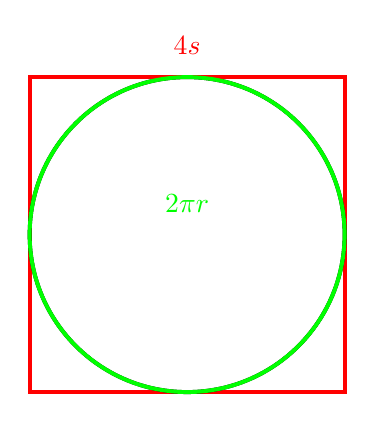
\begin{tikzpicture}
            \draw[line width = 0.5mm, red] (0,0) rectangle (4,4);
            \draw[line width = 0.5mm] (2,2) circle (2);
            \draw[line width = 0.5mm, red] (0,4) -- (4,4) node [label={[xshift=-2cm, yshift=0cm]$4s$}] {};
            \draw[line width = 0.5mm, green] (4,2) arc (0:360:2) node [label={[xshift=-2cm, yshift=0cm]$2\pi r$}] {};
            %\draw (2,2) -- (4,2) node[anchor=west] {r};
            % \draw[green] (2,2) -- (4,2) node [label={[xshift=-1cm, yshift=0.05cm]$r$}] {};
            % \draw[green] (4,2) arc (180:360:2);
        \end{tikzpicture}
    }
    \caption{Illustration showing that a square's perimeter corresponds to its incribed circle's circumference.}
    \label{fig:perimeter}
\end{figure}

\section*{Formulas as functions of $\theta$}
It is possible to express all the formulas as functions of $\theta$ by using a slightly different conversion fomula; however, the formula is only relevant for finding the arc lenght and area of a sector:
    \begin{align*}
        S &= C \cdot\dfrac{\pi}{2D} \mid  s=2r \\
        S(\theta) &= C \cdot\dfrac{\pi}{2D} \cdot \dfrac{\theta}{2\pi} \mid  s=2r 
    \end{align*}
This yields equation number (\ref{eq:theta}):
    \begin{align} \label{eq:theta}
        S(\theta) = C \cdot\dfrac{\theta}{4D} \mid s=2r
    \end{align}


\subsection*{Arc Lenght}
The formula for the arc length of a circle can be obtained from the perimeter formula of a square:
	\begin{align}
		C_{perimeter} = 4s && D =  2
	\end{align}	
The conversion formula is applied as normal, but the final result is multiplied by $\dfrac{\theta}{2\pi}$ as shown below:
	\begin{align*}
		S_{arcLength} &= C_{perimeter} \cdot\dfrac{\pi}{2D} \cdot \dfrac{\theta}{2\pi} \mid  s=2r \\
		&= 4s \cdot\dfrac{\pi}{2\cdot 2} \cdot \dfrac{\theta}{2\pi} \mid s=2r\\
		&= (2r) \cdot\dfrac{\theta}{2} \\
		&= \theta r
	\end{align*}

\subsection*{Sector Area}
The formula for the sector area of a circle can be obtained from the area formula of a square:
	\begin{align}
		C_{area} = s^{2} && D =  2
	\end{align}	
The conversion formula is applied as normal, but the final result is multiplied by $\dfrac{\theta}{2\pi}$ as shown below:
	\begin{align*}
		S_{sectorArea} &= C_{area} \cdot\dfrac{\pi}{2D} \cdot \dfrac{\theta}{2\pi} \mid  s=2r \\
		&= s^{2} \cdot\dfrac{\pi}{2\cdot 2} \cdot \dfrac{\theta}{2\pi} \mid s=2r\\
		&= (2r)^2 \cdot\dfrac{\theta}{8} \\
		&= 4r^2 \cdot\dfrac{\theta}{8} \\
		&= \dfrac{1}{2} \theta r^2
	\end{align*}

\section*{Formulas}

\subsection*{3D Shapes}
	\begin{align*}
		S_{volume} &= C_{volume} \cdot\dfrac{\pi}{2D} \mid  s=2r \\
		&= s^{3} \cdot\dfrac{\pi}{2\cdot 3} \mid s=2r\\
		&= (2r)^{3} \cdot\dfrac{\pi}{6} \\
		&= \dfrac{8\pi r^{3}}{6} \\
		&= \dfrac{4\pi r^{3}}{3} \\
	\end{align*}
	
		\begin{align*}
		S_{surfaceArea} &= C_{surfaceArea} \cdot\dfrac{\pi}{2D} \mid  s=2r \\
		&= 6s^{2} \cdot\dfrac{\pi}{2\cdot 3} \mid s=2r\\
		&= 6(2r)^{2} \cdot\dfrac{\pi}{6} \\
		&= 4\pi r^{2}
	\end{align*}

\subsection*{2D Shapes}
	\begin{align*}
		S_{area} &= C_{area} \cdot\dfrac{\pi}{2D} \mid  s=2r \\
		&= s^{2} \cdot\dfrac{\pi}{2\cdot 2} \mid s=2r\\
		&= (2r)^{2} \cdot\dfrac{\pi}{4} \\
		&= \dfrac{4\pi r^{2}}{4} \\
		&= \pi r^{2} \\
        S(\theta)_{sectorArea} &= \pi r^{2} \cdot \dfrac{\theta}{2\pi}  \\
        &= \dfrac{1}{2} \theta r^{2}  
	\end{align*}
	
	\begin{align*}
		S_{circumference} &= C_{perimeter} \cdot\dfrac{\pi}{2D} \mid  s=2r \\
		&= 4s \cdot\dfrac{\pi}{2\cdot 2} \mid s=2r\\
		&= 4(2r) \cdot\dfrac{\pi}{4} \\
		&= 2 \pi r \\
        S(\theta)_{arcLength} &= 2 \pi r \cdot \dfrac{\theta}{2\pi}  \\
        &= \theta r 
	\end{align*}

\end{document}
